% ============================================================
%  Module 2 — The Pin Factory
%  From Smith to Simulation · University of Edinburgh
% ============================================================
\documentclass[aspectratio=169, 10pt]{beamer}
\usetheme{metropolis}

% --- Edinburgh colours ----------------------------------------
\definecolor{UoERed}{HTML}{7A2318}
\definecolor{UoEGold}{HTML}{B8860B}
\definecolor{CodeBG}{HTML}{F7F3ED}
\definecolor{CodeFrame}{HTML}{D5C9B1}

\setbeamercolor{palette primary}{bg=UoERed, fg=white}
\setbeamercolor{frametitle}{bg=UoERed, fg=white}
\setbeamercolor{title separator}{fg=UoEGold}
\setbeamercolor{progress bar}{fg=UoEGold, bg=UoEGold!20}
\setbeamercolor{alerted text}{fg=UoERed}
\setbeamercolor{block title}{bg=UoERed!15, fg=UoERed}
\setbeamercolor{block body}{bg=UoERed!5}

% --- Packages -------------------------------------------------
\usepackage[T1]{fontenc}
\usepackage{lmodern}
\usepackage{amsmath, amssymb, mathtools}
\usepackage{listings}
\usepackage{graphicx, booktabs}
\usepackage{tikz}
\usetikzlibrary{arrows.meta, positioning, calc, decorations.pathreplacing}
\usepackage{hyperref}
\hypersetup{colorlinks=true, linkcolor=UoERed, urlcolor=UoERed!70!black}
\setbeamertemplate{navigation symbols}{}

\lstset{
  language=Python,
  basicstyle=\ttfamily\scriptsize,
  keywordstyle=\color{UoERed}\bfseries,
  commentstyle=\color{gray}\itshape,
  stringstyle=\color{UoEGold},
  backgroundcolor=\color{CodeBG},
  frame=single,
  rulecolor=\color{CodeFrame},
  numbers=none,
  breaklines=true,
  showstringspaces=false,
  tabsize=4,
  xleftmargin=4pt, xrightmargin=4pt,
  aboveskip=6pt, belowskip=4pt,
}

% Section title pages
\AtBeginSection[]{
  \begin{frame}
    \vfill\centering
    \usebeamerfont{title}\insertsectionhead\par
    \vfill
  \end{frame}
}

% ---- Title ---------------------------------------------------
\title{Module 2 --- The Pin Factory}
\subtitle{Division of Labour, Specialisation, and Trade}
\author{Dr Juan Zurita}
\institute{From Smith to Simulation\\
The University of Edinburgh~$\cdot$~School of Economics}
\date{}

\begin{document}

% =============================================================
\maketitle
% =============================================================

% -------------------------------------------------------------
\section{Part I --- The History}
% -------------------------------------------------------------

\begin{frame}{The Most Famous Factory in Economics}
\begin{columns}[T]
\column{0.58\textwidth}
\textit{The Wealth of Nations} opens not with grand theory but with a visit
to a \textbf{pin factory}:
\vspace{0.5em}
\begin{center}
\textit{``One man draws out the wire, another straights it,
a third cuts it, a fourth points it, a fifth grinds it
at the top for receiving the head\ldots''}\\[4pt]
--- Adam Smith, \textit{WN}, Book~I, Ch.~1
\end{center}
\vspace{0.5em}
Smith counted \alert{18 distinct operations} in making a single pin.
\column{0.38\textwidth}
\begin{block}{The Numbers}
\begin{description}
  \item[Alone] $\sim 20$ pins/day
  \item[Team of 10] $\sim 48{,}000$ pins/day
  \item[Per worker] $\sim 4{,}800$ pins/day
\end{description}
\vspace{0.3em}
A \textbf{240-fold increase} from specialisation alone.
\end{block}
\end{columns}
\end{frame}

\begin{frame}{The Pin Factory Pipeline}
\begin{center}
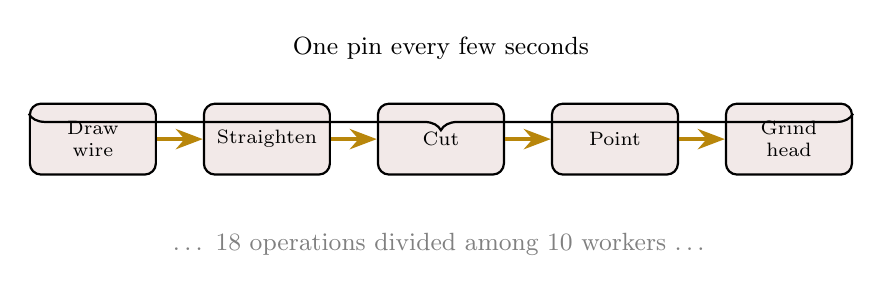
\begin{tikzpicture}[>=Stealth, thick, scale=0.85,
    worker/.style={draw, rounded corners, fill=UoERed!10,
                   minimum width=1.6cm, minimum height=0.9cm,
                   font=\scriptsize, align=center}]
  % Workers in pipeline
  \node[worker] (w1) at (0,0) {Draw\\wire};
  \node[worker] (w2) at (2.6,0) {Straighten};
  \node[worker] (w3) at (5.2,0) {Cut};
  \node[worker] (w4) at (7.8,0) {Point};
  \node[worker] (w5) at (10.4,0) {Grind\\head};

  \draw[->, line width=1.5pt, UoEGold] (w1) -- (w2);
  \draw[->, line width=1.5pt, UoEGold] (w2) -- (w3);
  \draw[->, line width=1.5pt, UoEGold] (w3) -- (w4);
  \draw[->, line width=1.5pt, UoEGold] (w4) -- (w5);

  \node[below=0.6cm of w3, font=\small, text=gray]
    {\ldots\ 18 operations divided among 10 workers \ldots};

  % Braces
  \draw[decorate, decoration={brace, amplitude=6pt, raise=4pt}]
    (w5.north east) -- (w1.north west)
    node[midway, above=12pt, font=\small] {One pin every few seconds};
\end{tikzpicture}
\end{center}
\vspace{0.5em}
The \textbf{pipeline} means each worker repeats one task all day.
The factory's throughput is determined by its \alert{bottleneck} ---
the slowest station.
\end{frame}

\begin{frame}{Why Does Specialisation Work?}
Smith identified three reasons:
\vspace{0.5em}
\begin{enumerate}
  \item \textbf{Skill improvement.}
        A worker who performs one task all day becomes extraordinarily
        good at it --- faster, more precise, more consistent.
  \item \textbf{Time saving.}
        No time wasted switching between tasks, moving between
        workstations, or picking up different tools.
  \item \textbf{Innovation.}
        Workers focused on a single task are more likely to invent
        machines or methods that improve it.
\end{enumerate}
\vspace{0.5em}
\begin{alertblock}{Key Quote}
Smith noted that many early industrial machines were invented by
\textit{workers themselves}, not by scientists.
\end{alertblock}
\end{frame}

\begin{frame}{The Extent of the Market}
\textit{``The division of labour is limited by the extent of the market.''}\\
\hfill --- Adam Smith, \textit{WN}, Book~I, Ch.~3
\vspace{1em}
\begin{columns}[T]
\column{0.48\textwidth}
\begin{block}{Small Village}
  \begin{itemize}
    \item Too few customers to justify 10 specialist pin-makers.
    \item Workers remain generalists.
    \item Low productivity persists.
  \end{itemize}
\end{block}
\column{0.48\textwidth}
\begin{block}{Large City / Seaport}
  \begin{itemize}
    \item Enough demand for specialised factories.
    \item Each worker masters one operation.
    \item Productivity soars.
  \end{itemize}
\end{block}
\end{columns}
\vspace{0.5em}
Specialisation requires \alert{scale}. Trade expands the market
and thereby deepens the division of labour.
\end{frame}

\begin{frame}{From Pin Factories to Nations}
Smith extended the logic of specialisation from factories to countries:
\vspace{0.5em}
\begin{itemize}
  \item Just as workers should specialise in what they do best,
        \textbf{nations} should trade rather than produce everything domestically.
  \item This idea was refined forty years later by \textbf{David Ricardo}
        (1772--1823).
\end{itemize}
\vspace{0.5em}
\begin{center}
\textit{``Under a system of perfectly free commerce, each country\\
naturally devotes its capital and labour to such employments\\
as are most beneficial to each.''}\\[4pt]
--- David Ricardo, \textit{Principles of Political Economy} (1817), Ch.~7
\end{center}
\end{frame}

\begin{frame}{Comparative Advantage: The Big Idea}
Ricardo proved something remarkable:
\vspace{0.5em}
\begin{block}{Absolute vs.\ Comparative Advantage}
  \begin{itemize}
    \item \textbf{Absolute advantage:} who produces a good with
          fewer resources.
    \item \textbf{Comparative advantage:} who produces a good at
          the lowest \alert{opportunity cost}.
  \end{itemize}
\end{block}
\vspace{0.5em}
Even if one country is better at producing \textit{everything},
both countries still gain from trade.
\vspace{0.5em}

What matters is not who is best overall but
\textbf{who gives up less} to produce each good.

\vspace{0.5em}
This is one of the most counterintuitive --- and most important ---
results in all of economics.
\end{frame}

\begin{frame}{Edinburgh Connection}
\begin{columns}[T]
\column{0.55\textwidth}
\begin{itemize}
  \item The pin factory Smith described was likely based on factories
        near \textbf{Edinburgh and Kirkcaldy}.
  \item In the 1760s Scotland's manufacturing was booming: linen,
        iron, metalwork.
  \item Edinburgh's merchants were embedded in international trade
        networks.
  \item The Old Town's closes and wynds were full of workshops where
        the division of labour was already visible in miniature.
\end{itemize}
\column{0.4\textwidth}
\begin{block}{Smith's Genius}
He saw in these ordinary workshops a
\textbf{universal principle}: specialisation creates wealth.
\end{block}
\end{columns}
\end{frame}

% -------------------------------------------------------------
\section{Part II --- The Computation}
% -------------------------------------------------------------

\begin{frame}[fragile]{Setting Up}
\begin{lstlisting}
import numpy as np
import matplotlib.pyplot as plt
\end{lstlisting}
\vspace{0.5em}
\begin{itemize}
  \item \texttt{numpy} --- numerical arrays and operations
  \item \texttt{matplotlib} --- plotting
\end{itemize}
\vspace{0.5em}
Today we will:
\begin{enumerate}
  \item Simulate Smith's pin factory
  \item Plot how productivity rises with specialisation
  \item Compute Ricardo's comparative advantage
  \item Visualise the gains from trade
\end{enumerate}
\end{frame}

\begin{frame}[fragile]{Simulating the Pin Factory (I)}
\textbf{Parameters:}
\begin{lstlisting}
n_steps = 18  # distinct operations to make a pin
working_day = 600  # minutes (10 hours)

# GENERALIST: slow at everything, switching costs
time_per_step_generalist = 3.0  # minutes per step
switching_cost = 1.0            # minutes lost per switch

# SPECIALIST: fast through practice, no switching
time_per_step_specialist = 0.5  # 6x faster
switching_cost_specialist = 0.0
\end{lstlisting}
\vspace{0.3em}
Key modelling choices:
\begin{itemize}
  \item Specialists are \textbf{6$\times$} faster per step (skill improvement)
  \item Switching between tasks wastes 1 minute each time
\end{itemize}
\end{frame}

\begin{frame}[fragile]{Simulating the Pin Factory (II)}
\begin{lstlisting}
# GENERALIST: time to make one pin
time_per_pin = n_steps * 3.0 + (n_steps - 1) * 1.0
pins_per_day_generalist = working_day / time_per_pin
# => 71 min/pin => 8.5 pins/day

# SPECIALIST TEAM: 10 workers in a pipeline
n_workers = 10
steps_per_worker = n_steps / n_workers  # ~1.8 steps
bottleneck_time = np.ceil(steps_per_worker) * 0.5
pins_per_day_total = working_day / bottleneck_time
# => 600 pins/day total, 60 per worker
\end{lstlisting}
\vspace{0.3em}
\begin{columns}[T]
\column{0.48\textwidth}
\begin{block}{Generalist}
71 min/pin $\Rightarrow$ \textbf{8.5} pins/day
\end{block}
\column{0.48\textwidth}
\begin{block}{Specialist Team}
1 min/pin $\Rightarrow$ \textbf{60} pins/worker/day
\end{block}
\end{columns}
\vspace{0.3em}
Even our simple model produces a \alert{7$\times$ gain}.
Smith observed 240$\times$ in practice --- the real world has
even stronger learning effects.
\end{frame}

\begin{frame}[fragile]{Productivity vs.\ Number of Specialists}
\begin{lstlisting}
def pins_per_worker(n_workers, n_steps=18,
    t_specialist=0.5, t_generalist=3.0,
    switch_cost=1.0, day=600):
    if n_workers == 1:
        time_per_pin = (n_steps * t_generalist
                        + (n_steps - 1) * switch_cost)
        return day / time_per_pin
    steps_each = max(1, n_steps / min(n_workers, n_steps))
    effective_time = t_specialist * steps_each**0.3
    bottleneck = np.ceil(steps_each) * effective_time
    total_pins = day / bottleneck
    return total_pins / n_workers
\end{lstlisting}
\vspace{0.3em}
The model captures:
\begin{itemize}
  \item \textbf{Pipeline throughput} limited by the bottleneck worker
  \item \textbf{Learning curve}: fewer steps per worker $\Rightarrow$
        faster per step ($\text{time} \propto \text{steps}^{0.3}$)
\end{itemize}
\end{frame}

\begin{frame}{Productivity Rises with Specialisation}
\begin{center}
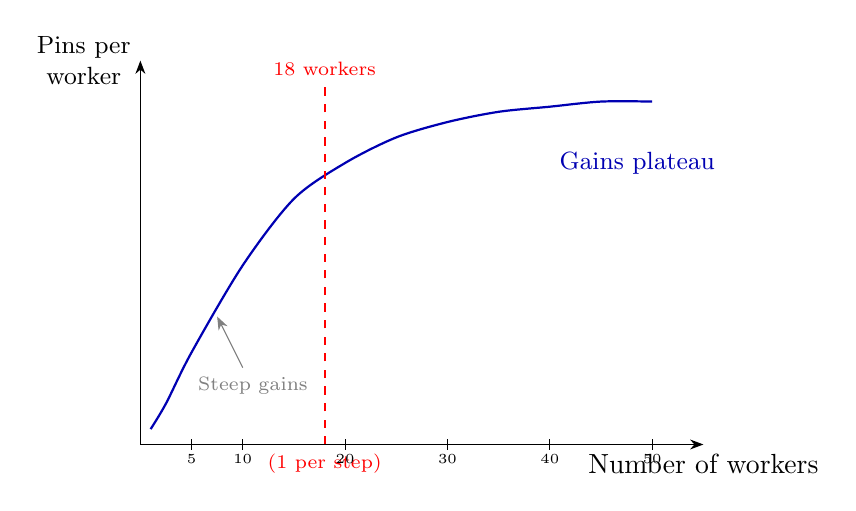
\begin{tikzpicture}[scale=0.65, >=Stealth]
  % Axes
  \draw[->] (0,0) -- (11,0) node[below] {Number of workers};
  \draw[->] (0,0) -- (0,7.5) node[left, align=center, font=\small]
    {Pins per\\worker};

  % Stylised curve: rapid rise, then plateau
  \draw[thick, blue!70!black] plot[smooth] coordinates
    {(0.2,0.3) (0.5,0.8) (1,1.8) (2,3.5) (3,4.8) (4,5.5) (5,6.0)
     (6,6.3) (7,6.5) (8,6.6) (9,6.7) (10,6.7)};

  % Vertical line at 18 workers
  \draw[dashed, red, thick] (3.6,0) -- (3.6,7)
    node[above, font=\scriptsize, text=red] {18 workers};
  \node[below, font=\scriptsize, text=red] at (3.6,0) {(1 per step)};

  % Annotations
  \node[right, font=\small, text=blue!70!black] at (8,5.5)
    {Gains plateau};
  \draw[->, gray] (2,1.5) -- (1.5,2.5);
  \node[below, font=\scriptsize, text=gray] at (2.2,1.5) {Steep gains};

  % Tick marks
  \foreach \x/\label in {1/5, 2/10, 4/20, 6/30, 8/40, 10/50}
    \draw (\x, -0.1) -- (\x, 0.1) node[below=2pt, font=\tiny] {\label};
\end{tikzpicture}
\end{center}
\vspace{0.3em}
Output per worker rises steeply as workers specialise in fewer steps.
Beyond 18 workers (one per step), gains plateau --- the division of
labour is \alert{limited by the number of distinct tasks}.
\end{frame}

\begin{frame}{Ricardo's Two-Country Model}
Consider \textbf{Scotland} and \textbf{Portugal} producing
\textbf{cloth} and \textbf{wine}:
\vspace{0.5em}
\begin{center}
\begin{tabular}{lcc}
\toprule
 & Hours per cloth & Hours per wine \\
\midrule
Scotland & 100 & 120 \\
Portugal & 90 & 80 \\
\bottomrule
\end{tabular}
\end{center}
\vspace{0.5em}
\begin{itemize}
  \item Portugal is better at producing \textit{both} goods
        (\textbf{absolute advantage} in everything).
  \item A naive analysis: Portugal has nothing to gain from trading
        with Scotland.
  \item Ricardo proved this wrong.
\end{itemize}
\end{frame}

\begin{frame}[fragile]{Computing Opportunity Costs}
\begin{lstlisting}
scotland_cloth, scotland_wine = 100, 120
portugal_cloth, portugal_wine = 90,  80

# Opportunity cost of 1 cloth (in wine forgone)
opp_cloth_scot = scotland_cloth / scotland_wine  # 0.833
opp_cloth_port = portugal_cloth / portugal_wine  # 1.125

# Opportunity cost of 1 wine (in cloth forgone)
opp_wine_scot = scotland_wine / scotland_cloth  # 1.200
opp_wine_port = portugal_wine / portugal_cloth  # 0.889
\end{lstlisting}
\vspace{0.3em}
\begin{columns}[T]
\column{0.48\textwidth}
\begin{block}{Scotland}
  1 cloth costs \textbf{0.833} wine\\
  1 wine costs 1.200 cloth
\end{block}
\column{0.48\textwidth}
\begin{block}{Portugal}
  1 cloth costs 1.125 wine\\
  1 wine costs \textbf{0.889} cloth
\end{block}
\end{columns}
\end{frame}

\begin{frame}{Who Has Comparative Advantage?}
\begin{center}
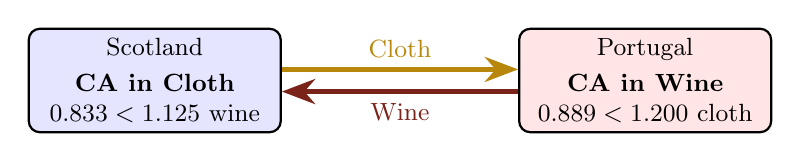
\begin{tikzpicture}[>=Stealth, thick,
    box/.style={draw, rounded corners, minimum width=3.2cm,
                minimum height=1.2cm, align=center, font=\small}]
  \node[box, fill=blue!10] (scot)
    {Scotland\\[2pt]\textbf{CA in Cloth}\\$0.833 < 1.125$ wine};
  \node[box, fill=red!10, right=3cm of scot] (port)
    {Portugal\\[2pt]\textbf{CA in Wine}\\$0.889 < 1.200$ cloth};

  \draw[->, line width=2pt, UoEGold]
    ([yshift=4pt]scot.east) -- ([yshift=4pt]port.west)
    node[midway, above, font=\small] {Cloth};
  \draw[<-, line width=2pt, UoERed]
    ([yshift=-4pt]scot.east) -- ([yshift=-4pt]port.west)
    node[midway, below, font=\small] {Wine};
\end{tikzpicture}
\end{center}
\vspace{0.5em}
\begin{itemize}
  \item Scotland gives up \textit{less wine} to make cloth
        $\Rightarrow$ CA in \textbf{cloth}.
  \item Portugal gives up \textit{less cloth} to make wine
        $\Rightarrow$ CA in \textbf{wine}.
  \item Each country specialises in the good where its
        opportunity cost is \alert{lower}.
\end{itemize}
\end{frame}

\begin{frame}{The Production Possibility Frontier}
Each country has $L = 1{,}000$ labour hours. The PPF shows all
feasible combinations of cloth and wine:
\[
  Q_{\text{wine}} = \frac{L - c_{\text{cloth}} \cdot Q_{\text{cloth}}}{c_{\text{wine}}}
\]
\begin{center}
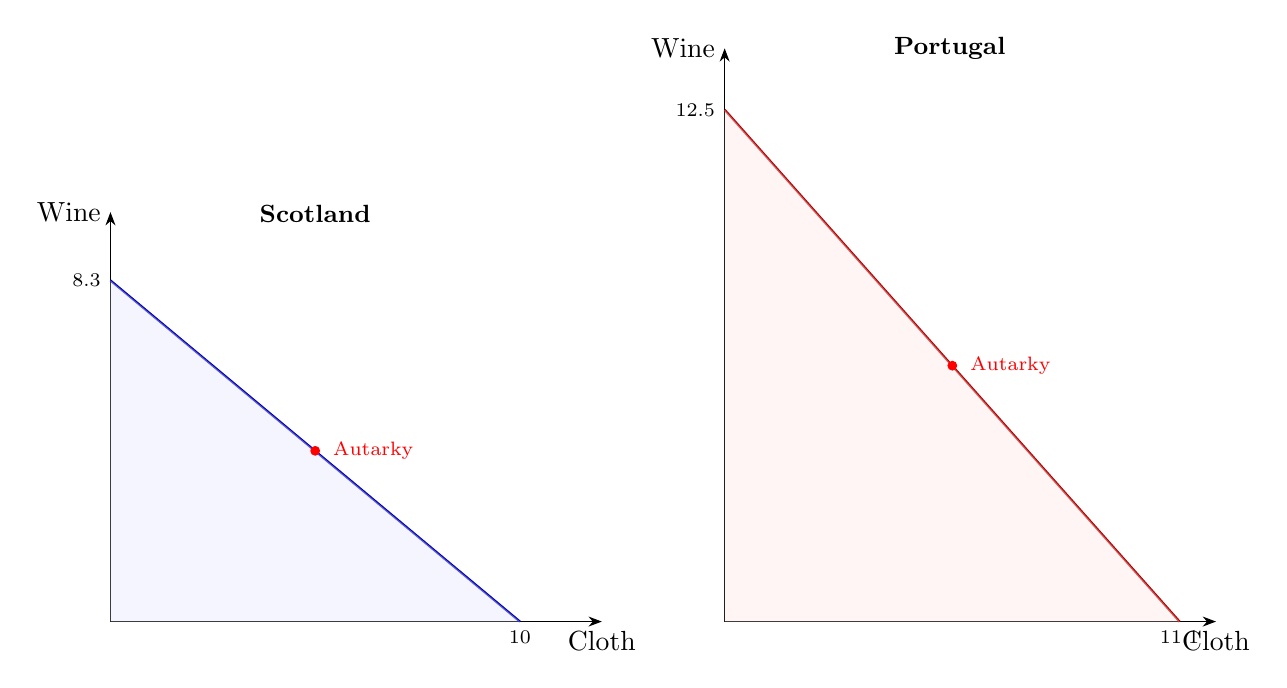
\begin{tikzpicture}[scale=0.52, >=Stealth]
  % --- Scotland ---
  \begin{scope}[shift={(0,0)}]
    \draw[->] (0,0) -- (12,0) node[below] {Cloth};
    \draw[->] (0,0) -- (0,10) node[left] {Wine};
    % Max cloth = 10, max wine = 8.33
    \draw[thick, blue!70!black] (0,8.33) -- (10,0);
    \fill[blue!10, opacity=0.4] (0,0) -- (0,8.33) -- (10,0) -- cycle;
    \node[below, font=\scriptsize] at (10,0) {10};
    \node[left, font=\scriptsize] at (0,8.33) {8.3};
    \node[above, font=\small\bfseries] at (5,9.5) {Scotland};
    % Autarky point
    \filldraw[red] (5,4.17) circle (3pt);
    \node[right, font=\scriptsize, red] at (5.2,4.17) {Autarky};
  \end{scope}
  % --- Portugal ---
  \begin{scope}[shift={(15,0)}]
    \draw[->] (0,0) -- (12,0) node[below] {Cloth};
    \draw[->] (0,0) -- (0,14) node[left] {Wine};
    % Max cloth = 11.11, max wine = 12.5
    \draw[thick, red!70!black] (0,12.5) -- (11.11,0);
    \fill[red!10, opacity=0.4] (0,0) -- (0,12.5) -- (11.11,0) -- cycle;
    \node[below, font=\scriptsize] at (11.11,0) {11.1};
    \node[left, font=\scriptsize] at (0,12.5) {12.5};
    \node[above, font=\small\bfseries] at (5.5,13.5) {Portugal};
    % Autarky point
    \filldraw[red] (5.56,6.25) circle (3pt);
    \node[right, font=\scriptsize, red] at (5.76,6.25) {Autarky};
  \end{scope}
\end{tikzpicture}
\end{center}
The PPF is a straight line because opportunity cost is constant (one input: labour).
\end{frame}

\begin{frame}[fragile]{PPF in Python}
\begin{lstlisting}
total_hours = 1000

def ppf(Q_cloth, cost_cloth, cost_wine, hours=1000):
    """Maximum wine given cloth production."""
    hours_left = hours - cost_cloth * Q_cloth
    return np.maximum(hours_left / cost_wine, 0)

scot_max_cloth = total_hours / 100   # 10.0
scot_max_wine  = total_hours / 120   # 8.33
port_max_cloth = total_hours / 90    # 11.11
port_max_wine  = total_hours / 80    # 12.5

cloth_s = np.linspace(0, scot_max_cloth, 100)
cloth_p = np.linspace(0, port_max_cloth, 100)

plt.plot(cloth_s, ppf(cloth_s, 100, 120), label='Scotland')
plt.plot(cloth_p, ppf(cloth_p, 90, 80),  label='Portugal')
plt.xlabel('Cloth'); plt.ylabel('Wine')
plt.legend(); plt.show()
\end{lstlisting}
\end{frame}

\begin{frame}[fragile]{Autarky: No Trade}
Suppose each country splits its 1,000 hours equally:
\begin{lstlisting}
half = 500  # hours on each good

scot_cloth_a = 500 / 100  # 5.0
scot_wine_a  = 500 / 120  # 4.17
port_cloth_a = 500 / 90   # 5.56
port_wine_a  = 500 / 80   # 6.25

world_cloth_a = 5.0 + 5.56   # 10.56
world_wine_a  = 4.17 + 6.25  # 10.42
\end{lstlisting}
\vspace{0.3em}
\begin{center}
\begin{tabular}{lccc}
\toprule
 & Cloth & Wine & \\
\midrule
Scotland & 5.00 & 4.17 & \\
Portugal & 5.56 & 6.25 & \\
\midrule
\textbf{World} & \textbf{10.56} & \textbf{10.42} & \\
\bottomrule
\end{tabular}
\end{center}
\end{frame}

\begin{frame}[fragile]{Specialisation + Trade}
Each country produces \textit{only} its comparative-advantage good:
\begin{lstlisting}
# Scotland: all labour on cloth
scot_cloth_t = 1000 / 100  # 10.0 cloth, 0 wine
# Portugal: all labour on wine
port_wine_t  = 1000 / 80   # 12.5 wine, 0 cloth

world_cloth_t = 10.0  # vs 10.56 autarky
world_wine_t  = 12.5  # vs 10.42 autarky
\end{lstlisting}
\vspace{0.3em}
\begin{center}
\begin{tabular}{lcc}
\toprule
 & Cloth & Wine \\
\midrule
\textbf{Autarky} & 10.56 & 10.42 \\
\textbf{Specialisation} & 10.00 & 12.50 \\
\midrule
\textbf{Change} & $-0.56$ & $\alert{+2.08}$ \\
\bottomrule
\end{tabular}
\end{center}
\vspace{0.3em}
Full specialisation produces much more wine at a small cost in cloth.
The \alert{net gain} is positive: the world is richer overall.
\end{frame}

\begin{frame}{Gains from Trade: The World PPF}
\begin{center}
\begin{tikzpicture}[scale=0.42, >=Stealth]
  % Axes
  \draw[->] (0,0) -- (24,0) node[below] {Total cloth};
  \draw[->] (0,0) -- (0,24) node[left] {Total wine};

  % Individual PPFs (dashed)
  \draw[dashed, blue!50, thick] (0,8.33) -- (10,0);
  \node[left, font=\tiny, blue!50] at (0,8.33) {8.3};
  \draw[dashed, red!50, thick] (0,12.5) -- (11.11,0);

  % World PPF with trade (kinked)
  % Point 1: all wine = 8.33+12.5 = 20.83, cloth = 0
  % Point 2: Scotland all cloth (10), Portugal all wine (12.5)
  % Point 3: all cloth = 10+11.11 = 21.11, wine = 0
  \draw[very thick, black] (0,20.83) -- (10,12.5) -- (21.11,0);
  \node[left, font=\scriptsize] at (0,20.83) {20.8};
  \node[below, font=\scriptsize] at (21.11,0) {21.1};

  % Autarky point
  \filldraw[red] (10.56, 10.42) circle (4pt);
  \node[above right, font=\small, red] at (10.56,10.42) {Autarky};

  % Trade point
  \filldraw[UoEGold] (10, 12.5) circle (5pt);
  \node[above right, font=\small, UoEGold!80!black] at (10.2,12.5)
    {Specialisation};

  % Arrow showing gain
  \draw[->, very thick, green!50!black]
    (10.56,10.42) -- (10,12.5);

  % Tick marks
  \foreach \x in {5,10,15,20}
    \draw (\x,-0.2) -- (\x,0.2) node[below=2pt, font=\tiny] {\x};
  \foreach \y in {5,10,15,20}
    \draw (-0.2,\y) -- (0.2,\y) node[left=2pt, font=\tiny] {\y};
\end{tikzpicture}
\end{center}
\vspace{0.3em}
The \textbf{world PPF with trade} lies outside the sum of individual PPFs.
Trade expands what the world can consume.
\end{frame}

\begin{frame}{Terms of Trade}
Specialisation creates a surplus. But who gets it?
That depends on the \alert{terms of trade}.
\vspace{0.5em}

For trade to benefit \textbf{both} countries, the price of cloth
(in wine) must lie between the two opportunity costs:
\[
  \underbrace{0.833}_{\text{Scotland's OC}} < \text{price of cloth}
  < \underbrace{1.125}_{\text{Portugal's OC}}
\]
\vspace{0.3em}
\begin{block}{Example: 1 cloth $= 1$ wine}
  Scotland produces 10 cloth, keeps 5, trades 5 for 5 wine.\\
  Portugal produces 12.5 wine, keeps 7.5, trades 5 for 5 cloth.\\[4pt]
  \textbf{Both} end up with more than under autarky.
\end{block}
\end{frame}

\begin{frame}[fragile]{Computing the Terms of Trade}
\begin{lstlisting}
terms_of_trade = 1.0  # 1 cloth = 1 wine

# Scotland: produces 10 cloth, keeps 5, trades 5
scot_keeps_cloth = 5
scot_gets_wine = 5 * terms_of_trade  # = 5.0
# Autarky: 5.0 cloth, 4.17 wine
# Trade:   5.0 cloth, 5.0 wine  => +0.83 wine!

# Portugal: produces 12.5 wine, sends 5, keeps 7.5
port_gets_cloth = 5
port_keeps_wine = 12.5 - 5.0  # = 7.5
# Autarky: 5.56 cloth, 6.25 wine
# Trade:   5.0 cloth, 7.5 wine  => +1.25 wine!
\end{lstlisting}
\vspace{0.3em}
\textbf{Ricardo's comparative advantage in action:}
both countries consume more than they could produce alone.
\end{frame}

% -------------------------------------------------------------
\section{Part III --- Exercises \& Discussion}
% -------------------------------------------------------------

\begin{frame}{Exercise 1: The Extent of the Market}
Smith wrote: \textit{``the division of labour is limited by the extent
of the market.''}
\vspace{0.5em}

A town consumes $D = 0.5 \times \text{population}$ pins per day.
\begin{itemize}
  \item Generalist: 10 pins/day (cost = wage\,/\,10 per pin).
  \item Specialist team of 10: 4{,}800 pins/day
        (cost = $10 \times \text{wage}\,/\,4{,}800$ per pin).
\end{itemize}
\vspace{0.3em}
\begin{enumerate}[(a)]
  \item What is the minimum population that justifies a specialist
        pin factory?
  \item Plot cost per pin under each mode as a function of daily
        demand. At what demand does specialisation become cheaper?
  \item Smith observed specialisation is most extreme in large cities
        and near seaports. Explain why in 2--3 sentences.
\end{enumerate}
\end{frame}

\begin{frame}{Exercise 2: Three-Country Comparative Advantage}
Extend Ricardo's model to three countries:
\vspace{0.3em}
\begin{center}
\begin{tabular}{lcc}
\toprule
 & Hours per cloth & Hours per wine \\
\midrule
Scotland & 100 & 120 \\
Portugal & 90 & 80 \\
France   & 110 & 90 \\
\bottomrule
\end{tabular}
\end{center}
Each country has 1{,}000 hours.
\vspace{0.3em}
\begin{enumerate}[(a)]
  \item Compute opportunity cost of cloth for all three countries.
        Who has strongest CA in cloth? In wine?
  \item Under autarky (50/50 split), what is world output?
  \item Under full specialisation (one country must split production),
        find the allocation that maximises world output.\\
        \textit{Hint: rank countries by opportunity cost of cloth.}
  \item Compute the gains from trade.
\end{enumerate}
\end{frame}

\begin{frame}{Exercise 3: Learning by Doing}
Smith's first reason for specialisation: practice improves skill.
Model with a \textbf{learning curve}:
\[
  t(n) = t_0 \cdot n^{-\beta}
\]
where $t(n)$ = time for the $n$-th repetition, $t_0$ = first attempt,
$\beta > 0$ = learning rate.
\vspace{0.3em}
\begin{enumerate}[(a)]
  \item A generalist performs each of 18 tasks 30 times/day.
        A specialist performs 1 task 540 times/day.
        Using $t_0 = 5$ min and $\beta = 0.3$, compute the
        average time per task for each.
  \item Plot $t(n)$ for $n = 1$ to $1{,}000$.
        When does the learning curve flatten?
  \item Compute total pins per day for a 10-worker specialist team
        with learning effects vs.\ a generalist with learning effects.
        How does the learning curve \alert{amplify} specialisation gains?
\end{enumerate}
\end{frame}

% -------------------------------------------------------------
\section{Quiz}
% -------------------------------------------------------------

\begin{frame}{Quiz --- Conceptual Questions (I)}
\textbf{Q1.} Which is \textbf{not} one of Smith's three reasons for
specialisation?
\begin{enumerate}[(a)]
  \item Workers become more skilled through repetition
  \item Workers save time by not switching between tasks
  \item Workers are paid lower wages when they specialise
  \item Specialised workers are more likely to invent improvements
\end{enumerate}
\vspace{0.5em}
\textbf{Q2.} Smith's pin factory showed that 10 workers with
division of labour could produce roughly:
\begin{enumerate}[(a)]
  \item 10 times more than 10 generalists
  \item 50 times more than 10 generalists
  \item 240 times more per worker than a generalist
  \item The same amount, but at lower cost
\end{enumerate}
\end{frame}

\begin{frame}{Quiz --- Conceptual Questions (II)}
\textbf{Q3.} ``The division of labour is limited by the extent of the
market'' means:
\begin{enumerate}[(a)]
  \item Markets should be regulated to prevent over-specialisation
  \item Specialisation only pays off with enough customers
  \item Large markets lead to monopolies
  \item Division of labour only works in manufacturing
\end{enumerate}
\vspace{0.5em}
\textbf{Q4.} Comparative advantage means:
\begin{enumerate}[(a)]
  \item A country can produce a good more cheaply in absolute terms
  \item A country gives up less of another good to produce one unit
  \item A country has more natural resources
  \item A country has lower wages
\end{enumerate}
\vspace{0.5em}
\textbf{Q5.} Portugal has absolute advantage in both goods. Scotland
has CA in cloth. Ricardo says:
\begin{enumerate}[(a)]
  \item Portugal should produce both; Scotland imports everything
  \item Scotland specialises in cloth, Portugal in wine; they trade
  \item Neither should trade
  \item Scotland should adopt Portuguese technology
\end{enumerate}
\end{frame}

\begin{frame}{Quiz --- Computational Questions (I)}
\textbf{Q6.} Scotland: 100 hrs/cloth, 120 hrs/wine.
Opportunity cost of 1~cloth is:
\begin{enumerate}[(a)]
  \item $100/120 = 0.833$ wine
  \item $120/100 = 1.2$ wine
  \item 100 wine
  \item 20 wine
\end{enumerate}
\vspace{0.5em}
\textbf{Q7.} A country with 1,000 hours, 50 hrs/cloth,
100 hrs/wine can produce at most:
\begin{enumerate}[(a)]
  \item 20 cloth or 10 wine
  \item 10 cloth or 20 wine
  \item 50 cloth or 100 wine
  \item 20 cloth or 20 wine
\end{enumerate}
\vspace{0.5em}
\textbf{Q8.} The PPF is a straight line when:
\begin{enumerate}[(a)]
  \item There are increasing returns to scale
  \item The opportunity cost is constant
  \item Both goods use the same inputs
  \item The country does not trade
\end{enumerate}
\end{frame}

\begin{frame}{Quiz --- Computational Questions (II)}
\textbf{Q9.} For trade to benefit both countries, the terms of trade
must lie:
\begin{enumerate}[(a)]
  \item Above both countries' opportunity costs
  \item Below both countries' opportunity costs
  \item Between the two countries' opportunity costs
  \item Equal to the average of their opportunity costs
\end{enumerate}
\vspace{0.5em}
\textbf{Q10.} Full specialisation with trade increases world output
because:
\begin{enumerate}[(a)]
  \item Each country produces what it is relatively best at,
        minimising total resource use
  \item Trade increases the total number of workers
  \item Specialisation eliminates diminishing returns
  \item Both countries adopt the same technology
\end{enumerate}
\vspace{1em}
\begin{center}
\small\textit{Answers: Q1(c), Q2(c), Q3(b), Q4(b), Q5(b),
Q6(a), Q7(a), Q8(b), Q9(c), Q10(a)}
\end{center}
\end{frame}

% -------------------------------------------------------------
\section{Key Takeaways}
% -------------------------------------------------------------

\begin{frame}{What We Learned This Week}
\begin{enumerate}
  \item Smith's \textbf{pin factory} (1776) showed that dividing labour
        into specialised tasks can increase productivity by orders of
        magnitude.
  \item Specialisation works through \textbf{skill improvement},
        \textbf{time saving}, and \textbf{innovation} --- but is
        limited by the extent of the market.
  \item Ricardo's \textbf{comparative advantage} (1817): even if one
        country is better at everything, both gain from trade based
        on \textit{opportunity cost}.
  \item The \textbf{PPF} visualises production trade-offs;
        specialisation and trade move the world \textit{beyond}
        individual frontiers.
  \item We can \textbf{simulate} these ideas: pin factory pipelines,
        opportunity cost calculations, and gains from trade ---
        all in a few lines of Python.
\end{enumerate}
\end{frame}

\begin{frame}{Further Reading}
\begin{itemize}
  \item Smith, A.\ \textit{The Wealth of Nations} (1776), Book~I, Chs.~1--3.\\
        Free at \url{https://www.econlib.org/library/Smith/smWN.html}
  \item Ricardo, D.\ \textit{Principles of Political Economy and Taxation}
        (1817), Ch.~7.
  \item Heilbroner, R.\ \textit{The Worldly Philosophers}, Ch.~3.
  \item Krugman, P.\ ``Ricardo's Difficult Idea'' (1996) --- a short essay
        on why people find comparative advantage so hard to accept.
\end{itemize}
\vspace{1em}
\begin{center}
\textbf{Next week:} Malthus, Ricardo, and the Limits to Growth ---\\
population dynamics, diminishing returns, and the Malthusian trap.
\end{center}
\end{frame}

\end{document}
